\documentclass[tikz,margin=3mm]{standalone}

\usepackage[T1]{fontenc}
\usepackage[utf8]{inputenc}
\usepackage{eulervm}
\usepackage{pgfplots}

\pgfplotsset{compat=newest}
\usetikzlibrary{patterns}
\usetikzlibrary{calc}
\usetikzlibrary{matrix}

\usepackage{color}

\definecolor{Comment}{RGB}{97,161,176}

\definecolor{btfGreen}{RGB}{51,160,44}
\definecolor{btfRed}{RGB}{190,60,90}

\definecolor{bleuUni}{RGB}{0, 157, 224}
\definecolor{marronUni}{RGB}{68, 58, 49}
\definecolor{grayMarronUni}{RGB}{60, 60, 60}
\definecolor{grayBleuUni}{RGB}{118, 118, 118}

\definecolor{bluecite}{HTML}{009DE0}

\definecolor{Paired-2}{RGB}{166,206,227}
\definecolor{Paired-1}{RGB}{31,120,180}
\definecolor{Paired-4}{RGB}{178,223,138}
\definecolor{Paired-3}{RGB}{51,160,44}
\definecolor{Paired-6}{RGB}{251,154,153}
\definecolor{Paired-5}{RGB}{227,26,28}
\definecolor{Paired-8}{RGB}{253,191,111}
\definecolor{Paired-7}{RGB}{255,127,0}
\definecolor{Paired-10}{RGB}{202,178,214}
\definecolor{Paired-9}{RGB}{106,61,154}
\definecolor{Paired-12}{RGB}{255,255,153}
\definecolor{Paired-11}{RGB}{177,89,40}
\definecolor{Accent-1}{RGB}{127,201,127}
\definecolor{Accent-2}{RGB}{190,174,212}
\definecolor{Accent-3}{RGB}{253,192,134}
\definecolor{Accent-4}{RGB}{255,255,153}
\definecolor{Accent-5}{RGB}{56,108,176}
\definecolor{Accent-6}{RGB}{240,2,127}
\definecolor{Accent-7}{RGB}{191,91,23}
\definecolor{Accent-8}{RGB}{102,102,102}
\definecolor{Spectral-1}{RGB}{158,1,66}
\definecolor{Spectral-2}{RGB}{213,62,79}
\definecolor{Spectral-3}{RGB}{244,109,67}
\definecolor{Spectral-4}{RGB}{253,174,97}
\definecolor{Spectral-5}{RGB}{254,224,139}
\definecolor{Spectral-6}{RGB}{255,255,191}
\definecolor{Spectral-7}{RGB}{230,245,152}
\definecolor{Spectral-8}{RGB}{171,221,164}
\definecolor{Spectral-9}{RGB}{102,194,165}
\definecolor{Spectral-10}{RGB}{50,136,189}
\definecolor{Spectral-11}{RGB}{94,79,162}
\definecolor{Set1-1}{RGB}{228,26,28}
\definecolor{Set1-2}{RGB}{55,126,184}
\definecolor{Set1-3}{RGB}{77,175,74}
\definecolor{Set1-4}{RGB}{152,78,163}
\definecolor{Set1-5}{RGB}{255,127,0}
\definecolor{Set1-6}{RGB}{255,255,51}
\definecolor{Set1-7}{RGB}{166,86,40}
\definecolor{Set1-8}{RGB}{247,129,191}
\definecolor{Set1-9}{RGB}{153,153,153}
\definecolor{Set2-1}{RGB}{102,194,165}
\definecolor{Set2-2}{RGB}{252,141,98}
\definecolor{Set2-3}{RGB}{141,160,203}
\definecolor{Set2-4}{RGB}{231,138,195}
\definecolor{Set2-5}{RGB}{166,216,84}
\definecolor{Set2-6}{RGB}{255,217,47}
\definecolor{Set2-7}{RGB}{229,196,148}
\definecolor{Set2-8}{RGB}{179,179,179}
\definecolor{Dark2-1}{RGB}{27,158,119}
\definecolor{Dark2-2}{RGB}{217,95,2}
\definecolor{Dark2-3}{RGB}{117,112,179}
\definecolor{Dark2-4}{RGB}{231,41,138}
\definecolor{Dark2-5}{RGB}{102,166,30}
\definecolor{Dark2-6}{RGB}{230,171,2}
\definecolor{Dark2-7}{RGB}{166,118,29}
\definecolor{Dark2-8}{RGB}{102,102,102}
\definecolor{Reds-1}{RGB}{255,245,240}
\definecolor{Reds-2}{RGB}{254,224,210}
\definecolor{Reds-3}{RGB}{252,187,161}
\definecolor{Reds-4}{RGB}{252,146,114}
\definecolor{Reds-5}{RGB}{251,106,74}
\definecolor{Reds-6}{RGB}{239,59,44}
\definecolor{Reds-7}{RGB}{203,24,29}
\definecolor{Reds-8}{RGB}{165,15,21}
\definecolor{Reds-9}{RGB}{103,0,13}
\definecolor{Greens-1}{RGB}{247,252,245}
\definecolor{Greens-2}{RGB}{229,245,224}
\definecolor{Greens-3}{RGB}{199,233,192}
\definecolor{Greens-4}{RGB}{161,217,155}
\definecolor{Greens-5}{RGB}{116,196,118}
\definecolor{Greens-6}{RGB}{65,171,93}
\definecolor{Greens-7}{RGB}{35,139,69}
\definecolor{Greens-8}{RGB}{0,109,44}
\definecolor{Greens-9}{RGB}{0,68,27}
\definecolor{Blues-1}{RGB}{247,251,255}
\definecolor{Blues-2}{RGB}{222,235,247}
\definecolor{Blues-3}{RGB}{198,219,239}
\definecolor{Blues-4}{RGB}{158,202,225}
\definecolor{Blues-5}{RGB}{107,174,214}
\definecolor{Blues-6}{RGB}{66,146,198}
\definecolor{Blues-7}{RGB}{33,113,181}
\definecolor{Blues-8}{RGB}{8,81,156}
\definecolor{Blues-9}{RGB}{8,48,107}


\begin{document}
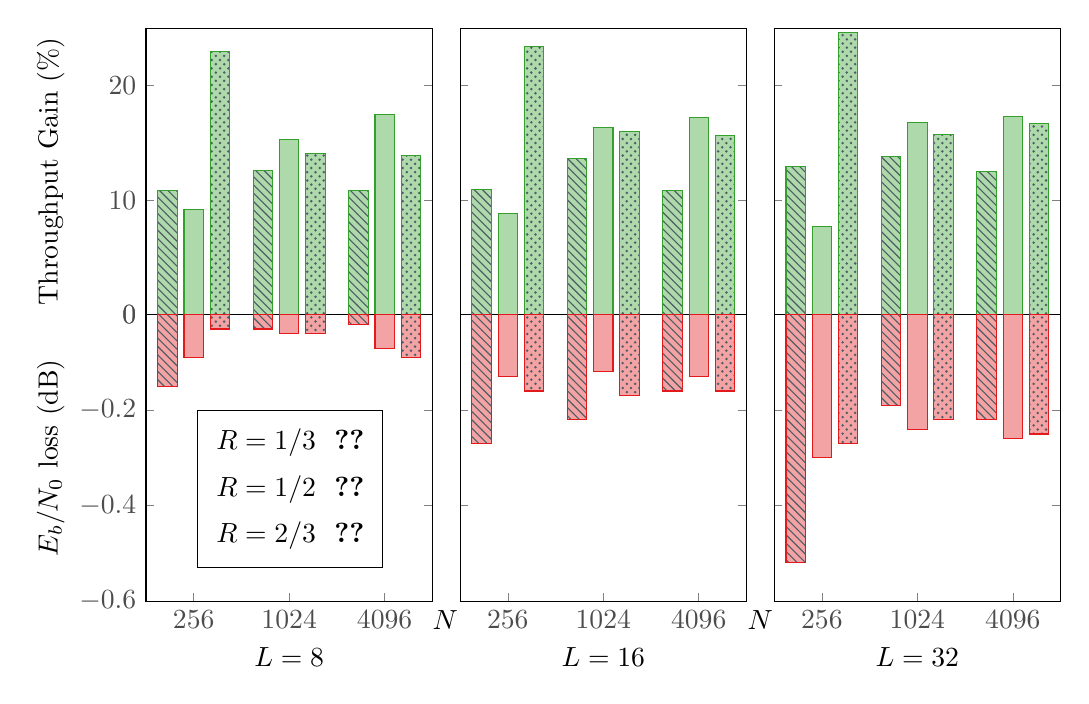
\begin{tikzpicture}


\pgfplotsset{major tick length=3}
\begin{axis}[%
name=plot1,
width=0.30\textwidth,
height=0.3\textwidth,
xticklabel style={black!70}, yticklabel style={black!70},
area legend,
scale only axis,
xmin=0,
xmajorticks=false,
xmax=12,
ymin=0,
ymax=25,
axis x line*=top,
ylabel={Throughput Gain (\%)},
y label style={at={(-0.25,0.5)}},
bar width=7pt,
]
\addplot[ybar,fill=Paired-3!40,draw=Paired-3,postaction={pattern color = black!80!Paired-1!70, pattern=north west  lines}] plot coordinates{
(0.90,10.8)
(4.90,12.6)
(8.90,10.8)
};
\addplot[ybar,fill=Paired-3!40,draw=Paired-3] plot coordinates{
(2,9.2)
(6,15.3)
(10,17.5)
};
\addplot[ybar,fill=Paired-3!40,draw=Paired-3,postaction={pattern color = black!80!Paired-1!70, pattern=crosshatch  dots}] plot coordinates{
(3.1,23.0)
(7.1,14.1)
(11.1,13.9)
};
\end{axis}

\begin{axis}[
name=plot2,
area legend,
scale only axis,
at={($(plot1.south)$)},anchor=north,
width=0.30\textwidth,
height=0.3\textwidth,
xticklabel style={black!70}, yticklabel style={black!70},
xmin=0,
xmax=12,
xtick={2,6,10},
xticklabels={$256$,$1024$,$4096$},
xlabel={$L=8$},
ymin=-0.6,
ymax=0,
ylabel={$E_b/N_0$ loss (dB)},
bar width=7pt,
y label style={at={(-0.25,0.5)}},
legend style={draw=black,fill=white,legend cell align=left, at={(0.75,0.6)}}
]
% \legend{$R=1/3$,$R=1/2$,$R=2/3$};
\coordinate (legend) at (6.05,-0.2);

\addplot[ybar,fill=Paired-5!40,draw=Paired-5,postaction={pattern color = black!80!Paired-1!70, pattern=north west  lines}] plot coordinates{
( 0.90, -0.15)
( 4.90, -0.03)
(8.90, -0.02)
};

\addplot[ybar,fill=Paired-5!40,draw=Paired-5] plot coordinates{
( 2, -0.09)
( 6, -0.04)
(10, -0.07)
};

\addplot[ybar,fill=Paired-5!40,draw=Paired-5,postaction={pattern color = black!80!Paired-1!70, pattern=crosshatch  dots}] plot coordinates{
( 3.1, -0.03)
( 7.1, -0.04)
(11.1, -0.09)
};

\end{axis}


\begin{axis}[%
name=plot3,
width=0.30\textwidth,
height=0.3\textwidth,
xticklabel style={black!70}, yticklabel style={black!70},
at={($(plot1.east)+ (10,0) $)},anchor=west,
area legend,
scale only axis,
xmin=0,
xmajorticks=false,
yticklabels={,,},
xmax=12,
ymin=0,
ymax=25,
axis x line*=top,
y label style={at={(-0.1,0.5)}},
bar width=7pt,
]
\addplot[ybar,fill=Paired-3!40,draw=Paired-3,postaction={pattern color = black!80!Paired-1!70, pattern=north west  lines}] plot coordinates{
(0.90,10.9)
(4.90,13.6)
(8.90,10.8)};
\addplot[ybar,fill=Paired-3!40,draw=Paired-3] plot coordinates{
(2,8.8)
(6,16.3)
(10,17.2)};
\addplot[ybar,fill=Paired-3!40,draw=Paired-3,postaction={pattern color = black!80!Paired-1!70, pattern=crosshatch  dots}] plot coordinates{
(3.1,23.4)
(7.1,16.0)
(11.1,15.6)};
\end{axis}

\begin{axis}[
name=plot4,
area legend,
scale only axis,
at={($(plot2.east)+ (10,0) $)},anchor=west,
width=0.30\textwidth,
yticklabels={,,},
height=0.3\textwidth,
xticklabel style={black!70}, yticklabel style={black!70},
xmin=0,
xmax=12,
xtick={2,6,10},
xticklabels={$256$,$1024$,$4096$},
xlabel={$L=16$},
ymin=-0.6,
ymax=0,
bar width=7pt,
y label style={at={(-0.1,0.5)}},
legend style={fill=white}
]

\addplot[ybar,fill=white,draw=black,postaction={pattern color = black!80!Paired-1!70, pattern=north west  lines}] plot coordinates{
(1,0)
};
\label{plot:R_1_3}

\addplot[ybar,fill=white,draw=black] plot coordinates{
(1,0)
};
\label{plot:R_1_2}

\addplot[ybar,fill=white,draw=black,postaction={pattern color = black!80!Paired-1!70, pattern=crosshatch  dots}] plot coordinates{
(1,0)
};
\label{plot:R_2_3}

\addplot[ybar,fill=Paired-5!40,draw=Paired-5,postaction={pattern color = black!80!Paired-1!70, pattern=north west  lines}] plot coordinates{
(0.90, -0.27)
(4.90, -0.22)
(8.90, -0.16)};

\addplot[ybar,fill=Paired-5!40,draw=Paired-5] plot coordinates{
(2, -0.13)
(6, -0.12)
(10, -0.13)};

\addplot[ybar,fill=Paired-5!40,draw=Paired-5,postaction={pattern color = black!80!Paired-1!70, pattern=crosshatch  dots}] plot coordinates{
(3.1, -0.16)
(7.1, -0.17)
(11.1, -0.16)};

\end{axis}


\begin{axis}[%
name=plot5,
width=0.30\textwidth,
height=0.3\textwidth,
xticklabel style={black!70}, yticklabel style={black!70},
at={($(plot3.east)+ (10,0) $)},anchor=west,
area legend,
scale only axis,
xmin=0,
xmajorticks=false,
xmax=12,
ymin=0,
ymax=25,
axis x line*=top,
yticklabels={,,},
y label style={at={(-0.1,0.5)}},
bar width=7pt,
]
\addplot[ybar,fill=Paired-3!40,draw=Paired-3,postaction={pattern color = black!80!Paired-1!70, pattern=north west  lines}] plot coordinates{
(0.90,12.9)
(4.90,13.8)
(8.90,12.5)};
\addplot[ybar,fill=Paired-3!40,draw=Paired-3] plot coordinates{
(2 ,7.7)
(6 ,16.8)
(10,17.3)};
\addplot[ybar,fill=Paired-3!40,draw=Paired-3,postaction={pattern color = black!80!Paired-1!70, pattern=crosshatch  dots}] plot coordinates{
(3.1,24.6)
(7.1,15.7)
(11.1,16.7)};
\end{axis}

\begin{axis}[
name=plot6,
area legend,
scale only axis,
at={($(plot4.east)+ (10,0) $)},anchor=west,
width=0.30\textwidth,
height=0.3\textwidth,
xticklabel style={black!70}, yticklabel style={black!70},
xmin=0,
xmax=12,
xtick={2,6,10},
xticklabels={$256$,$1024$,$4096$},
xlabel={$L=32$},
ymin=-0.6,
ymax=0,
bar width=7pt,
yticklabels={,,},
y label style={at={(-0.1,0.5)}},
legend style={fill=white}
]

\addplot[ybar,fill=Paired-5!40,draw=Paired-5,postaction={pattern color = black!80!Paired-1!70, pattern=north west  lines}] plot coordinates{
(0.90, -0.52)
(4.90, -0.19)
(8.90, -0.22)};

\addplot[ybar,fill=Paired-5!40,draw=Paired-5] plot coordinates{
(2, -0.30)
(6, -0.24)
(10, -0.26)};

\addplot[ybar,fill=Paired-5!40,draw=Paired-5,postaction={pattern color = black!80!Paired-1!70, pattern=crosshatch  dots}] plot coordinates{
(3.1, -0.27)
(7.1, -0.22)
(11.1, -0.25)};

\end{axis}

  \matrix [
      draw,
      matrix of nodes,
      anchor=north,
      fill=white
  ] at (legend) {
      $R = 1/3$ & \ref{plot:R_1_3}  \\
      $R = 1/2$ & \ref{plot:R_1_2}  \\
      $R = 2/3$ & \ref{plot:R_2_3}  \\
  };
\node at (3.8,-3.88) {$N$};
\node at (7.8,-3.88) {$N$};

\end{tikzpicture}%
\end{document}